\chapter{Конструкция безвинтового подводного робота с внутренними роторами}\label{ch:ch3}

\section{Описание конструкции безвинтового подводного робота с внутренними роторами}

Безвинтовой подводный робот является мобильным роботом в форме эллипсоида и представляет собой сборную конструкцию (рисунок \ref{constr_BPR}). Основой конструкции является оболочка 1 в форме эллипсоида, составленная из двух одинаковых половин 2, присоединенных друг к другу по экваториальной плоскости с помощью дискообразной перегородки – платформы 3. Размер эллипсоида по большей оси составляет 300 мм, по меньшей – 200 мм. Толщина оболочки (3 мм) и применяемый материал обеспечивают необходимую прочность при погружении и перемещении робота. Соединение полуоболочек и платформы обеспечивает герметичность внутренней полости.

\begin{figure}[h]
	\centering
	\includegraphics[width=0.9\linewidth]{constr_BPR.png}%
	\caption{Конструкция и корпусные элементы экспериментальной модели безвинтового подводного робота}
	\label{constr_BPR}
\end{figure}

Внутри корпуса робота установлены три пары роторов (далее система роторов) таким образом, что оси роторов расположены под углом $90^\circ$ по отношению друг к другу. Ось одной из пар роторов направлена вдоль оси вращения эллипсоида, а две другие пары расположены в экваториальной плоскости. Обеспечение точного управляющего воздействия $\omega_k (t)$ осуществляется с помощью встроенных в приводы датчиков обратной связи (энкодеров). Система роторов подводного робота включает пару роторов большего размера 4, установленных симметрично относительно платформы 3 на одной общей оси, и двух других пар роторов меньшего размера 5, расположенных (по направлениям осей) перпендикулярно первой паре и перпендикулярно друг другу в экваториальной плоскости. Оси малых роторов выполнены отдельно для каждого маховика и установлены соосно на некотором расстоянии друг от друга. Малые роторы соединены кинематически попарно с помощью промежуточных (дополнительных) осей и зубчатых пар таким образом, что их вращение происходит также, как если бы они были на одной общей оси.

Для приведения в движение системы роторов каждая из пар роторов оснащена высокомоментными мотор-редукторами, которые установлены в соответствующих опорах на платформе. В пространствах между большими и малыми роторами симметрично с двух сторон относительно платформы на панелях смонтированы модули питания 6, управления и связи. Передача данных для управления движением и получением дополнительной информации о состоянии системы может осуществляться по проводному и беспроводному вариантам связи.

Размещение узлов на платформе выполнено таким образом, чтобы в максимальной степени обеспечить симметричное расположение масс относительно геометрического центра тела, а также по возможности обеспечить минимальное отклонение центра масс от геометрического.

Для погружения робот оснащен механизмом регулировки плавучести. Он состоит из двух одинаковых модулей плавучести 7, размещенных и закрепленных внутри полуоболочек в наиболее удаленных частях относительно платформы. Модули плавучести имеют в своем составе лопастной насос 8 с приводом 9 на основе микроэлектродвигателя с редуктором. Полости насоса --- воздушная и жидкостная имеют каналы 10, соединяющие их соответственно с внутренней полостью и внешней средой.

Для контроля глубины робот оснащен двумя датчиками давления. Так же для определения ориентации робот имеет датчик MPU9250, который включает в себя трехосевой акселерометр, трехосевой гироскоп и трехосевой магнитометр.


Разработанная конструкция мобильного робота в форме эллипсоида имеет следующие характеристики: масса оболочки: $2.923$ кг; момент инерции маховиков большего размера: $7.491\cdot10^{-4}$ кг$\cdot$м; масса маховиков большего размера: $0.903$ кг;	момент инерции маховиков меньшего размера: $0.491\cdot10-4$ кг$\cdot$м;	масса маховиков меньшего размера: $0.337$ кг.

Фотографии робота в сборе и без половины оболочки представлены на рисунке \ref{Photo_BPR}.

\begin{figure}[h]
	\centering
	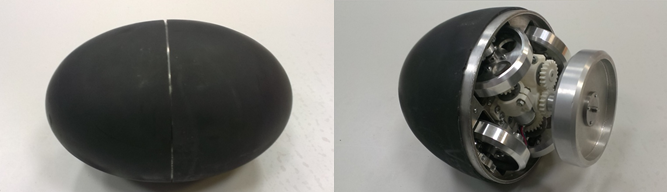
\includegraphics[width=0.9\linewidth]{Photo_BPR.png}%
	\caption{Фотографии безвинтового подводного робота}
	\label{Photo_BPR}
\end{figure}

\section{Описание системы управления безвинтового подводного робота с внутренними роторами}

В полученных математических моделях управление роторами задается в виде вектора внутреннего гиростатического момента $\bK$. Для управления отдельным двигателем разработана следующая схема (см. рисунок \ref{Control_system}).

\begin{figure}[h]
	\centering
	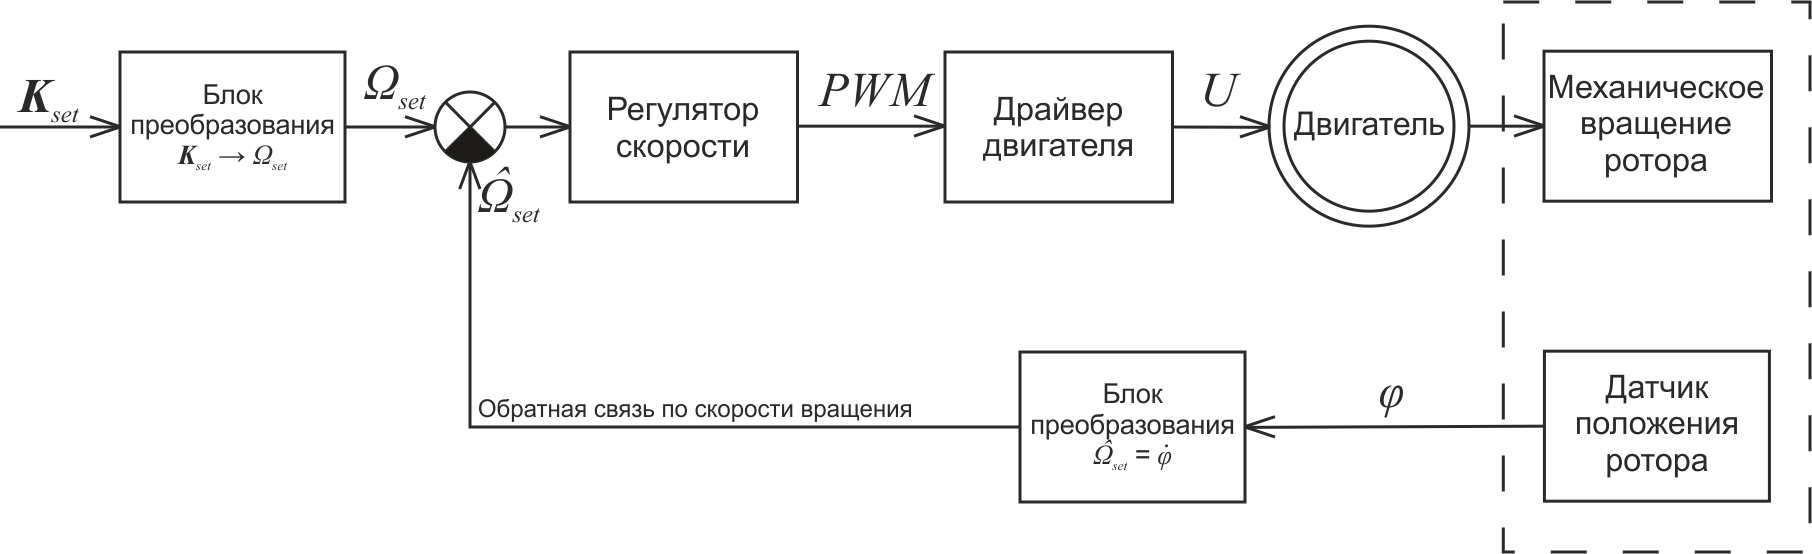
\includegraphics[width=0.9\linewidth]{Control_system.png}%
	\caption{Схема управления отдельным двигателем, где $\bK_{set}$ -- вектор внутреннего гиростатического момента; $\bOm_{set}$ -- угловая скорость вращения двигателя; $\hat{\bOm}_{set}$ -- фактическая скорость вращения двигателя; $PWM$ -- широтно-импульсная модуляция, рассчитаная для заданной скорости вращения; $U$ -- напряжение, подаваемое на двигатель; $\varphi$ -- фактическое положение ротора}
	\label{Control_system}
\end{figure}

Структурная схема системы управления безвинтового подводного робота, представлена на рисунке \ref{str_scheme}.

\begin{figure}[h!]
	\begin{center}
		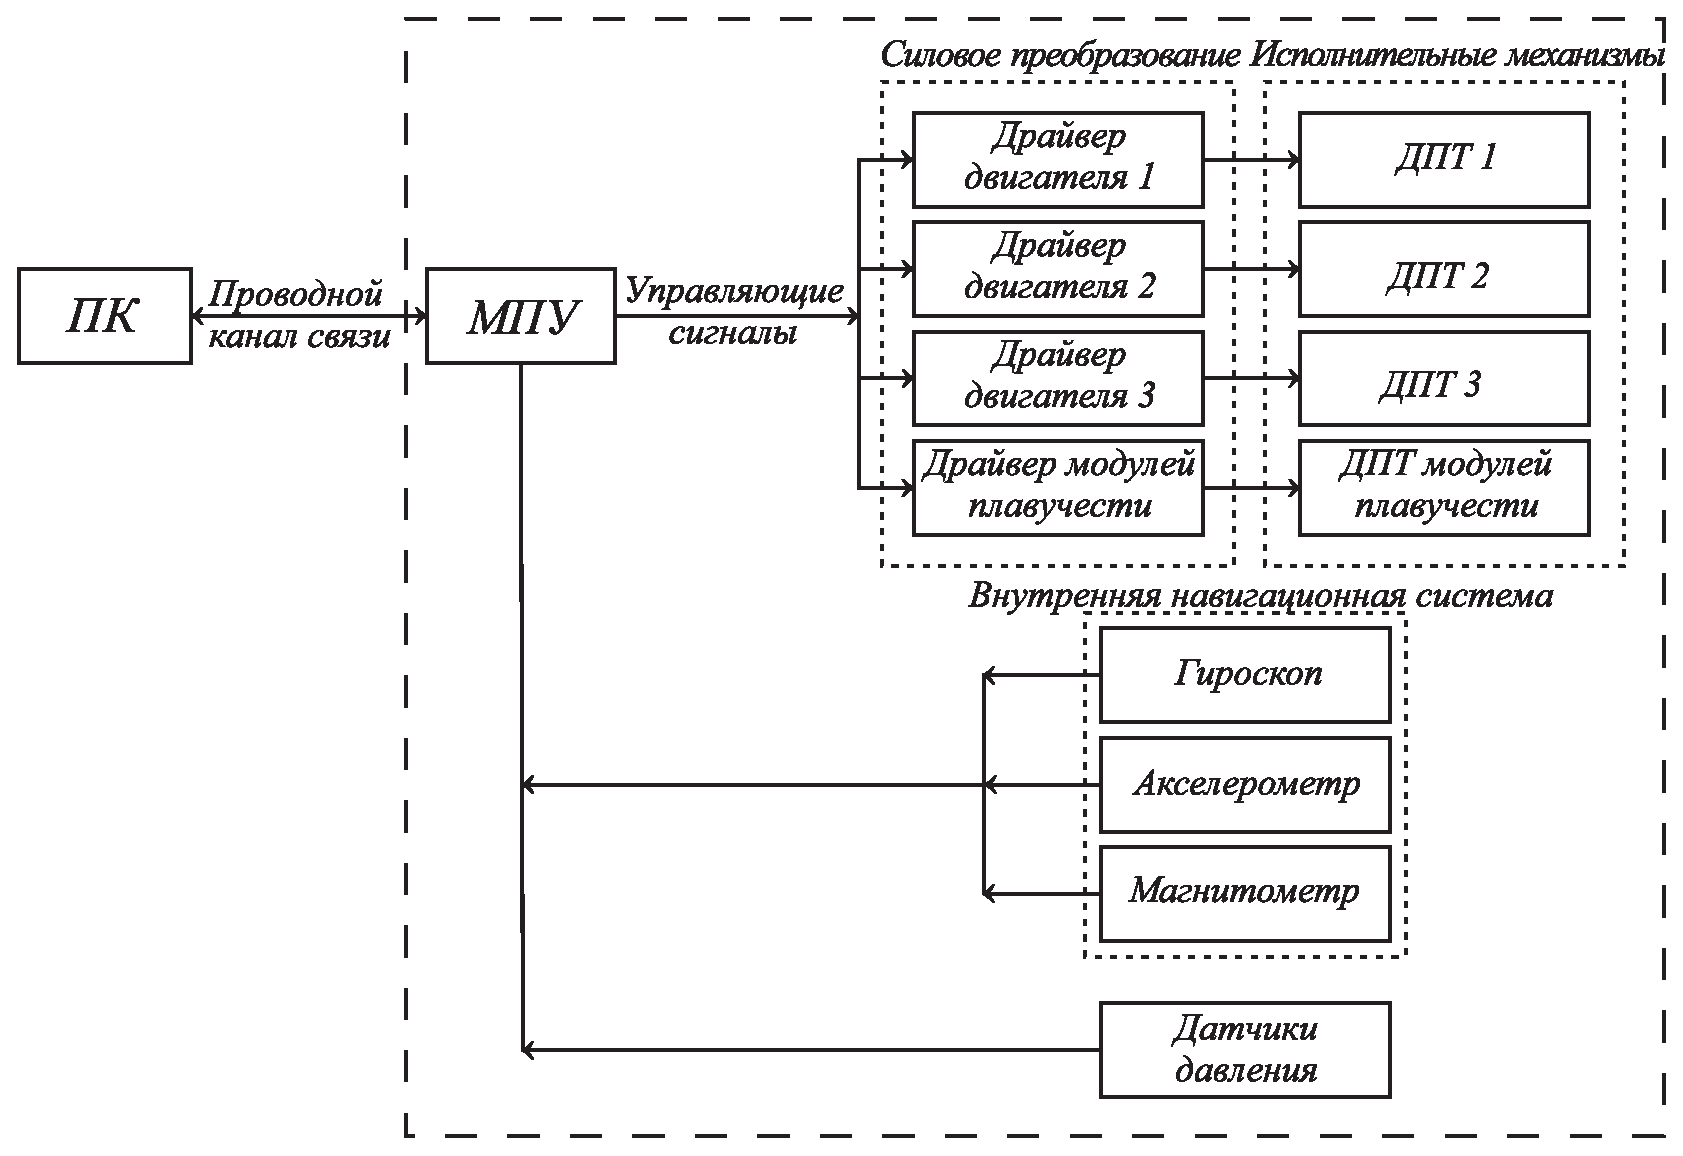
\includegraphics[width=0.8\linewidth]{StrSchemeBPR.eps}
		\caption{Структурная схема системы управления подводным роботом} \label{str_scheme}
	\end{center}
\end{figure}

Оператор на персональном компьютере (ПК, см. рисунок \ref{str_scheme}) задает команды управления подводным роботом. Команды передаются на микропроцессорное устройство (МПУ) по проводному или безпроводному (если робот находится на поверхности воды) каналу связи и представляют собой закодированные скорости вращения роторов или двигателей модулей плавучести. Далее микропроцессор обрабатывает полученные данные и формирует управляющий сигнал, подаваемый на драйверы двигателей или драйверы модулей плавучести, которые, в свою очередь, подают напряжение нужной формы и амплитуды на двигатели постоянного тока (ДПТ) или модули плавучести. Плата управления также содержит трехосевые акселерометр, гироскоп и магнитометр, которые являются внутренней навигационной системой робота и служат для определения ориентации робота. В качестве датчиков глубины погружения робота, используются датчики давления, расположенные в полюсах эллипсоида. Использование информации с данных датчиков в качестве обратной связи позволит регулировать плавучесть на заданной глубине погружения.


Система управления основана на микроконтроллере LPC1768. Плата управления с электронными компонентами, разработанная для робота представлена на рисунке~\ref{PCB_BPR}

\begin{figure}[h!]
	\begin{center}
		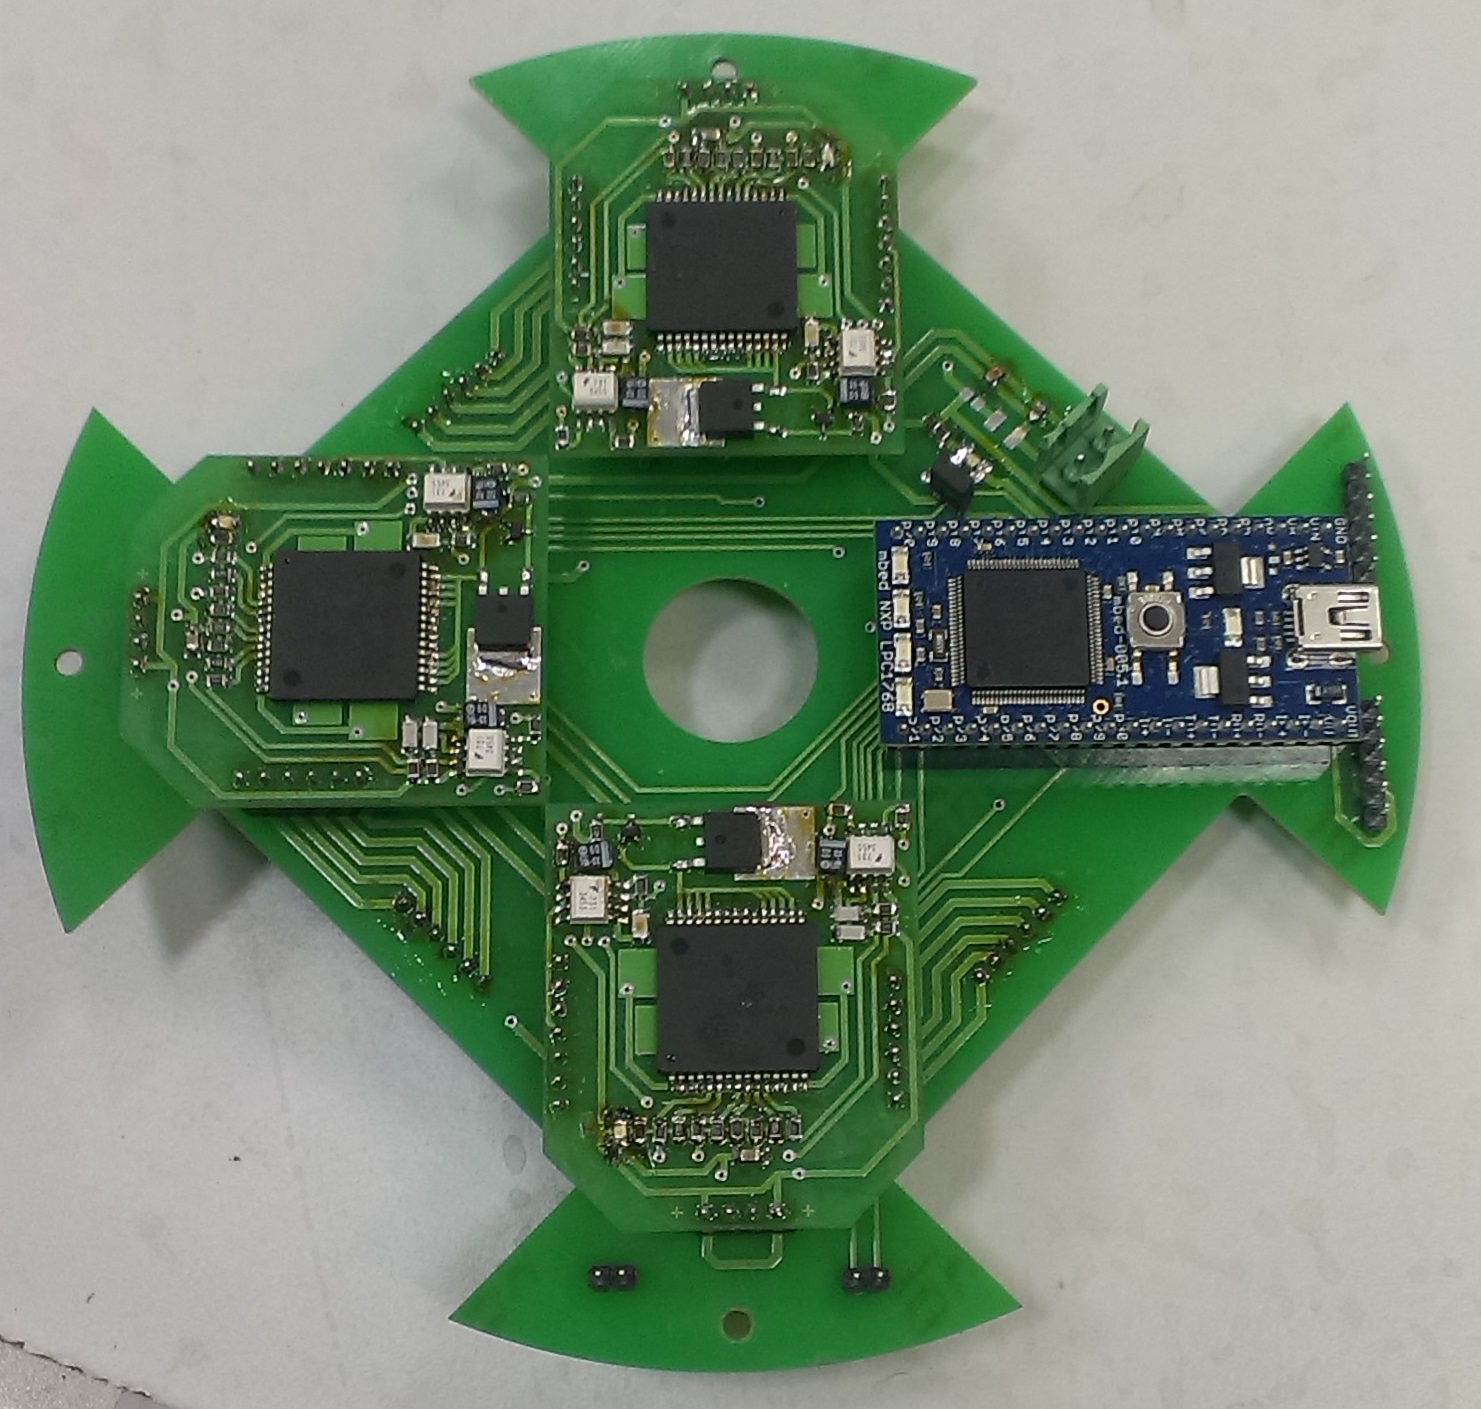
\includegraphics[width=0.8\linewidth]{PCB_BPR.png}
		\caption{Плата управления безвинтового подводного робота} \label{PCB_BPR}
	\end{center}
\end{figure}

Управление осуществляется с персонального компьютера (ПК), для которого было разработано специальное программное обеспечение. Для управления роботом необходимо задать направления и скорости вращения каждого из роторов, а также время разгона до заданной скорости. Отдельно осуществляется управление модулями плавучести, которые отвечают за погружение робота.



\clearpage